\chapter{Bilder}
\label{chap:bilder}
Für qualitativ hochwertige Dokumente sollten möglichst hochauflösende Bilder oder SVG-Grafiken (\url{https://de.wikipedia.org/wiki/Scalable_Vector_Graphics}) verwendet werden, da besonders im Druck schlechte Auflösungen negativ hervorstechen.

Bilder können in die \textit{Fließumgebung} \texttt{figure} gepackt werden. Für Positionierungsoptionen siehe \autoref{sec:fliessumgebungen}. Das Bild innerhalb der Fließumgebung \texttt{figure} wird mit dem Befehl \mintinline{latex}{\includegraphics[options]{path}} durch das Paket \texttt{graphicx} eingefügt. In \texttt{options} sollte immer die Option \mintinline{latex}{width=\columnwidth} gesetzt werden. Bei einem einspaltigen Layout kann alternativ zu \mintinline{latex}{\columnwidth} auch \mintinline{latex}{\textwidth} verwendet werden. Diese Breitenangaben können auch durch Modifikatoren verändert werden. So kann das Bild zum Beispiel auf 70\,\% der Textbreite mit der Option \mintinline{latex}{width=0.7\textwidth} skaliert werden.

\begin{showcase}
    \begin{code}{latex}
        \begin{figure}[Hhtbp] % Here!, here, top, bottom, page
            \centering % ← zentriert das Bild
            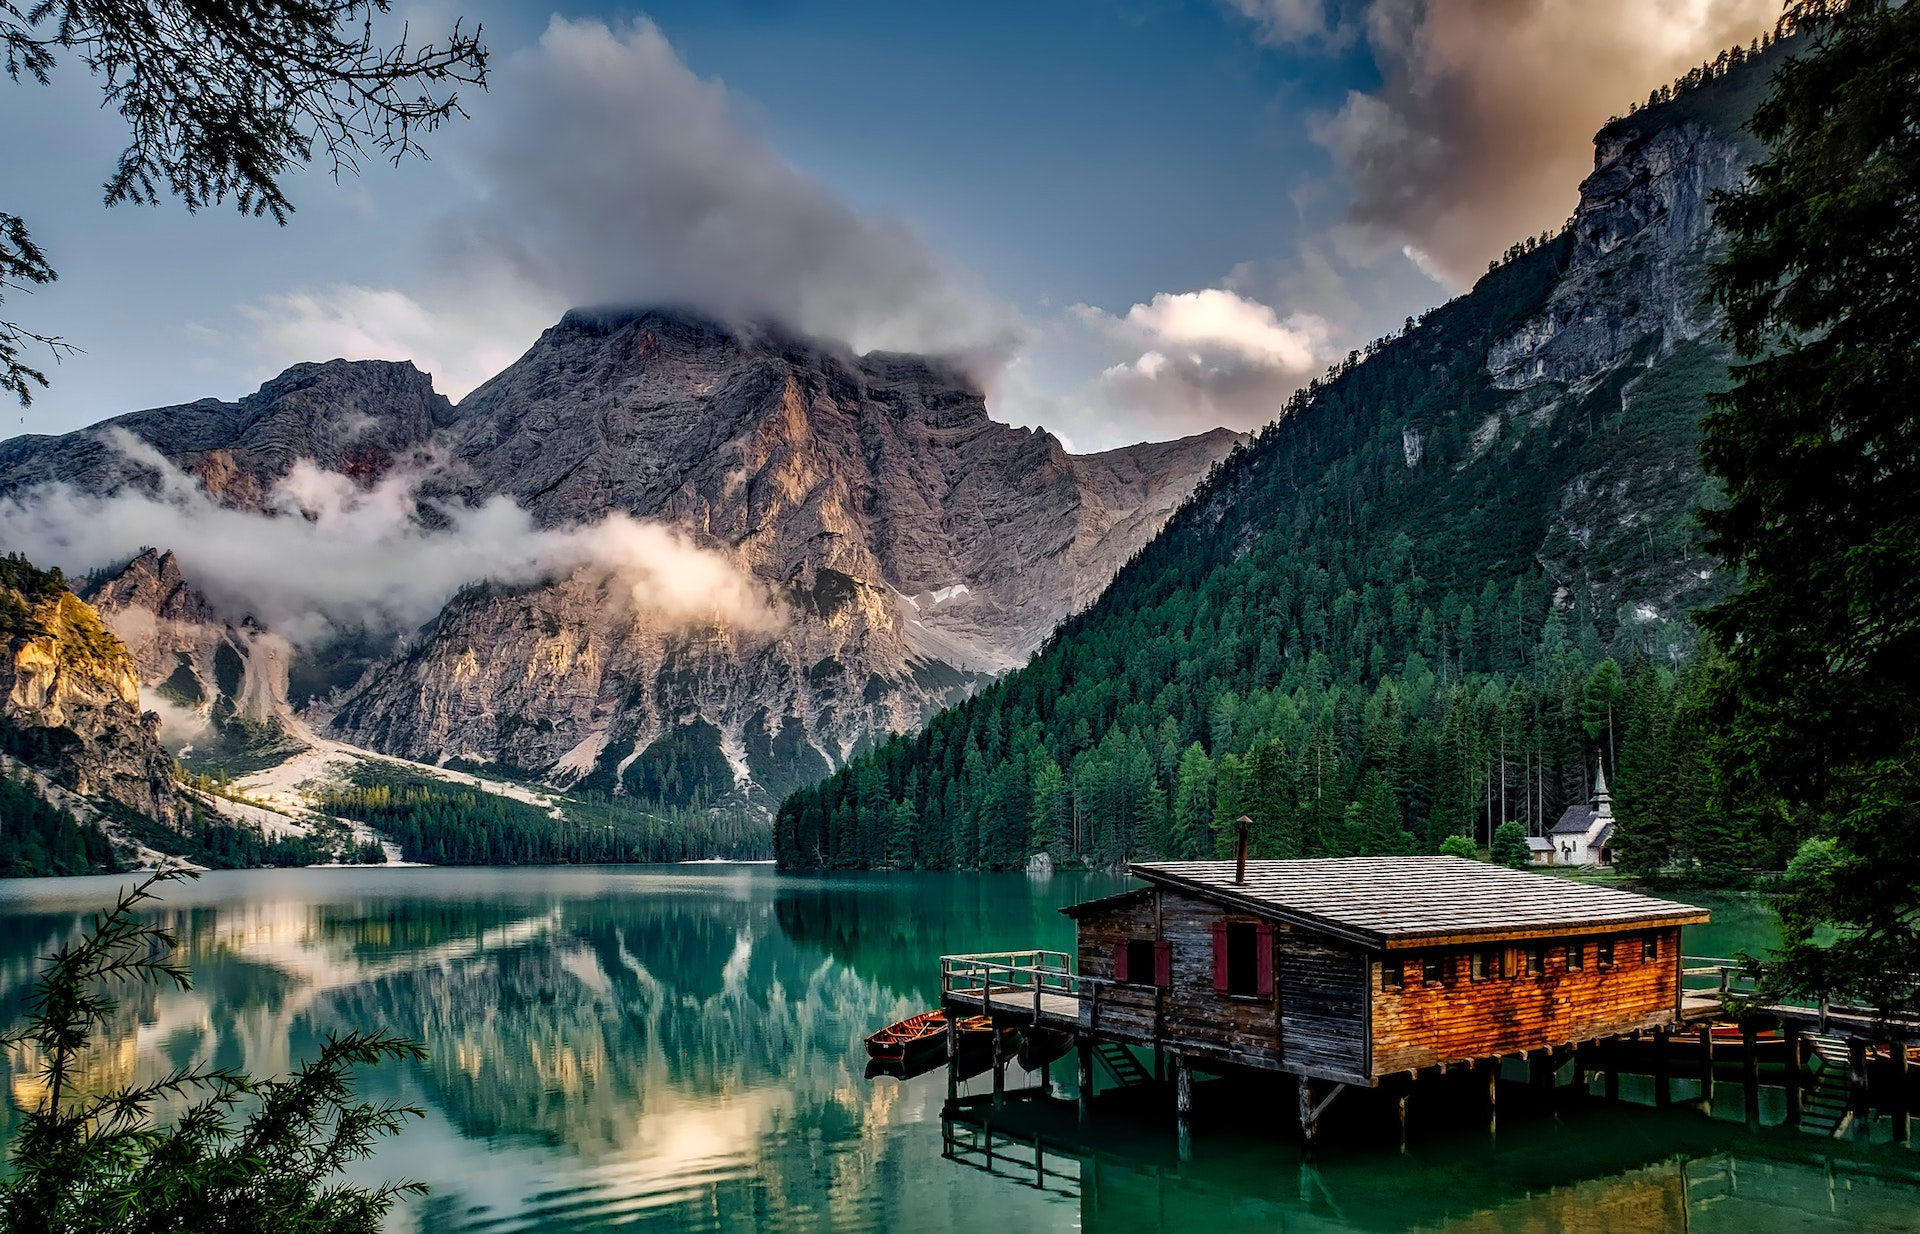
\includegraphics[width=0.7\columnwidth]{assets/images/bilder/pexels-pixabay-147411.jpg}
            \caption{Holzhaus am Gebirgssee}
            \label{fig:holzhaus-am-gebirgssee}
        \end{figure}
    \end{code}
    \tcblower
    \begin{center}
        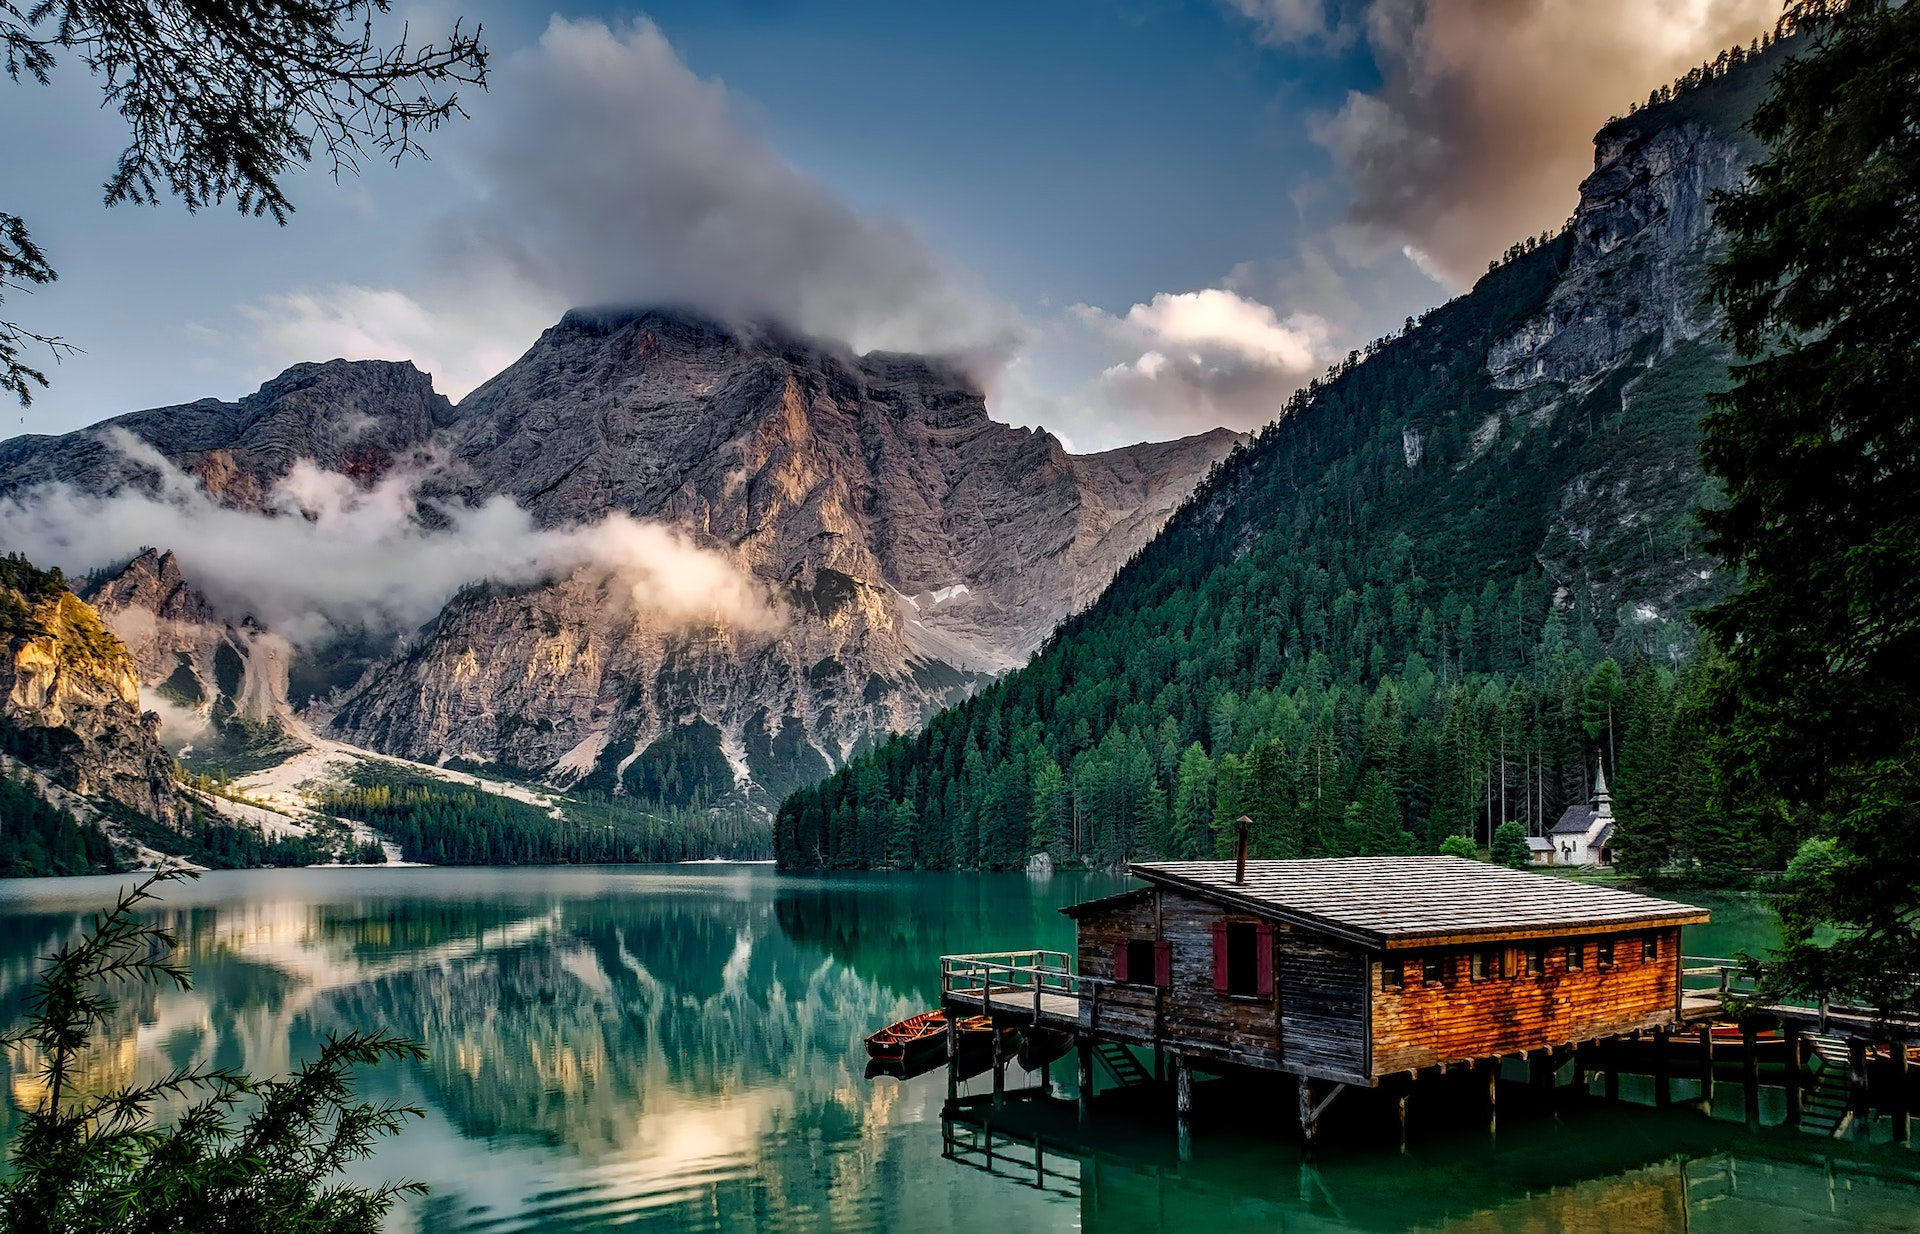
\includegraphics[width=0.7\columnwidth]{assets/images/bilder/pexels-pixabay-147411.jpg}
        \captionof{figure}{Holzhaus am Gebirgssee}
    \end{center}
\end{showcase}

\section{Vektorgrafiken (SVG)}
Sollen komplexe Informationen auf klare und ansprechende Weise wie in Infografiken oder Diagrammen dargestellt werden, eignen sich Vektorgrafiken. Im Gegensatz zu rasterbasierten Formaten (wie JPEG oder PNG) behalten SVG-Grafiken ihre Qualität und Schärfe unabhängig von der Zoomstufe oder Größe. Um SVG-Grafiken in \LaTeX-Dokumente einzufügen, gibt es verschiedene Ansätze, welche im folgenden kurz vorgestellt werden.

\subsection{Konvertierung zu PDF oder EPS}
Werden Grafiken zum Beispiel mit \textit{draw.io}\footnote{\url{https://www.drawio.com/}}, \textit{Inkscape}\footnote{\url{https://inkscape.org/de/}} oder anderen Werkzeugen selbst erstellt, empfiehlt es sich diese auch immer als PDF zu exportieren. Beim Export sollte darauf geachtet werden, dass die Größe des Bildes nur die gezeichneten Inhalte umfasst. Ich persönlich markiere dafür alle gezeichneten Elemente und exportiere nur die Auswahl, wobei es hier verschiedene Möglichkeiten gibt, da beim Markieren Teile des Bildes übersehen werden können. Die als PDF exportierten Bilder können wie normale Bilder mit dem Befehl \mintinline{latex}{\includegraphics[options]{path/to/file.pdf}} in das Dokument eingebettet werden.

\begin{showcase}
    \begin{code}{latex}
        \begin{figure}
            \centering
            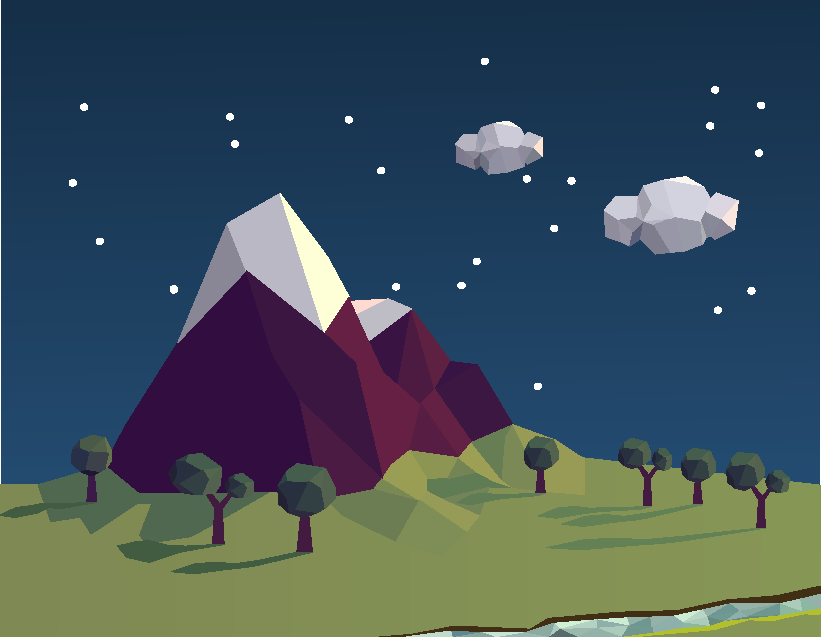
\includegraphics[width=0.5\columnwidth]{assets/images/bilder/landscape.pdf}
            \caption{Landschaft als PDF-Grafik}
            \label{fig:landschaft-als-pdf-grafik}
        \end{figure}        
    \end{code}
    \tcblower
    \begin{center}
        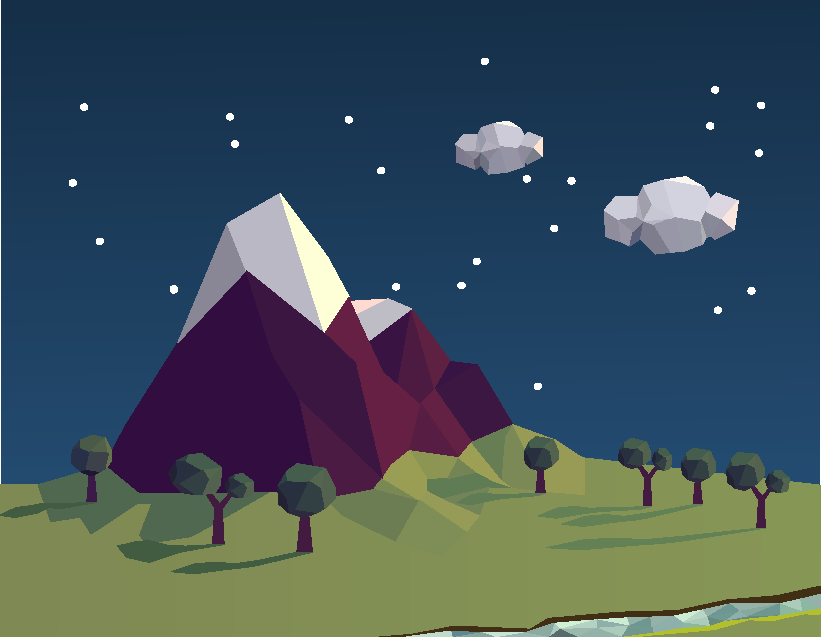
\includegraphics[width=0.5\columnwidth]{assets/images/bilder/landscape.pdf}
        \captionof{figure}{Landschaft als PDF-Grafik}
        \label{fig:landschaft-als-pdf-grafik}
    \end{center}  
\end{showcase}

\subsection{Direkte Verwendung von SVG-Grafiken}
Bei der direkten Verwendung werden die SVG-Grafiken mit den Befehl \mintinline{latex}{\includesvg[options]{path/to/file.svg}} zum Beispiel innerhalb eine Fließumgebung (siehe \autoref{sec:fliessumgebungen}) geladen. \textbf{Durch das Paket wird Inkscape ausgeführt}, weswegen es notwendig ist dieses Programm auf dem Rechner installiert zu haben. Außerdem ist es notwendig für die Ausführung mit z.\,B. \texttt{latexmk} die Option \texttt{-shell-escape} hinzuzufügen. Weitere Informationen für die lokale Einrichtung des Computers zur Verwendung dieses Templates sind auf \url{https://github.com/blackapple113/H-BRS-Thesisvorlage}.\todo{Setup Guide in README}

\begin{showcase}
    \begin{code}{latex}
        \begin{figure}
            \centering
            \includesvg[width=0.5\columnwidth]{assets/images/bilder/landscape.svg}
            \caption{Landschaft als SVG-Grafik}
            \label{fig:landschaft-als-svg-grafik}
        \end{figure}
    \end{code}
    \tcblower
    \begin{center}
        \includesvg[width=0.5\columnwidth]{assets/images/bilder/landscape.svg}
        \captionof{figure}{Landschaft als SVG-Grafik}
        \label{fig:landschaft-als-svg-grafik}
    \end{center}
\end{showcase}

\subsection{Vergleich SVG- vs. PDF-Grafik}
\label{subsec:vergleich-svg-vs-pdf-grafik}
Werden SVG-Grafiken direkt in \LaTeX verwendet werden sie in ein \LaTeX verständliches Format umgewandelt. Dabei können ungewollte Formatierungsprobleme innerhalb der Grafik auftreten. Als Beispiel werden im Folgenden zwei Diagramme gezeigt. Das Diagramm auf der linken Seite wurde als PDF importiert und das Diagramm auf der rechten Seite als SVG-Grafik. Es sei gesagt, dass die klasse \texttt{hbrs-thesis} schon einige Optionen für die bessere Verwendung von SVG-Grafiken eingestellt hat. Dennoch kann es, wie im Beispiel gezeigt, zu Problemen kommen.

\begin{figure}[H]
    \begin{minipage}[c]{0.48\columnwidth}
        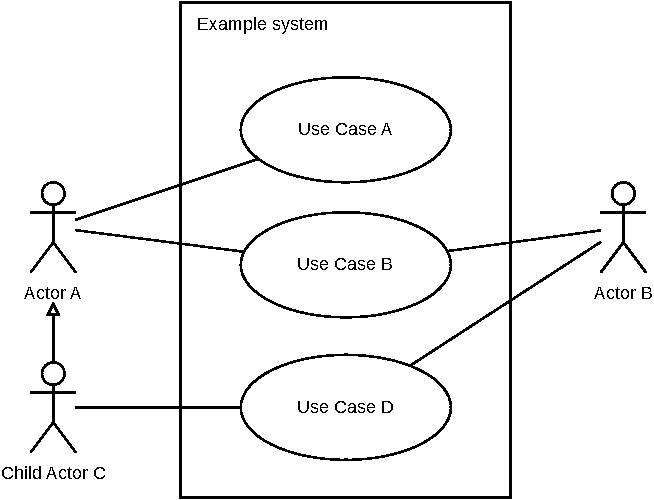
\includegraphics[width=\linewidth]{assets/images/bilder/UML-exmaple.pdf}
        \subcaption{PDF-Grafik}
        \label{subfig:pdf-grafik}
    \end{minipage}
    \hfill
    \begin{minipage}[c]{0.48\columnwidth}
        \includesvg[width=\linewidth]{assets/images/bilder/UML-example.svg}
        \subcaption{SVG-Grafik}
        \label{subfig:svg-grafik}
    \end{minipage}       
    \caption{SVG- vs. PDF-Grafik} 
\end{figure}

Die in diesem Beispiel gezeigten Unterschiede sind so gering, dass sie bei der ersten Kontrolle vielleicht gar nicht auffallen. Bei genauerer Betrachtung kann man erkennen, dass die Beschriftungen der einzelnen Aktoren in der SVG-Grafik nicht ausgeschrieben sind. Es fehlen also relevante Informationen, die in der PDF-Grafik enthalten sind. Trotzdem handelt es sich bei der PDF-Datei um eine Vektorgrafik, welche also keinen Qualitätsverlust aufweist.

\section{Teilbilder}
Wie in \autoref{subsec:vergleich-svg-vs-pdf-grafik} als Vergleichsabbildung zwischen SVG- und PDF-Grafiken verwendet, müssen manchmal mehrere Bilder nebeneinander platziert werden. Diese können unabhängig voneinander Beschriftet werden oder als Teil der übergeordneten Fließumgebung. Um Bilder nebeneinander platzieren zu können, wird die Umgebung \texttt{minipage} (siehe \autoref{sec:minipage}) verwendet. Im Folgenden ein paar Beispiele für die Anordnung von Bildern in einer Reihe.

\begin{showcase}
    \begin{code}{latex}
        \begin{figure}
            \centering
            \begin{minipage}[c]{0.49\columnwidth}
                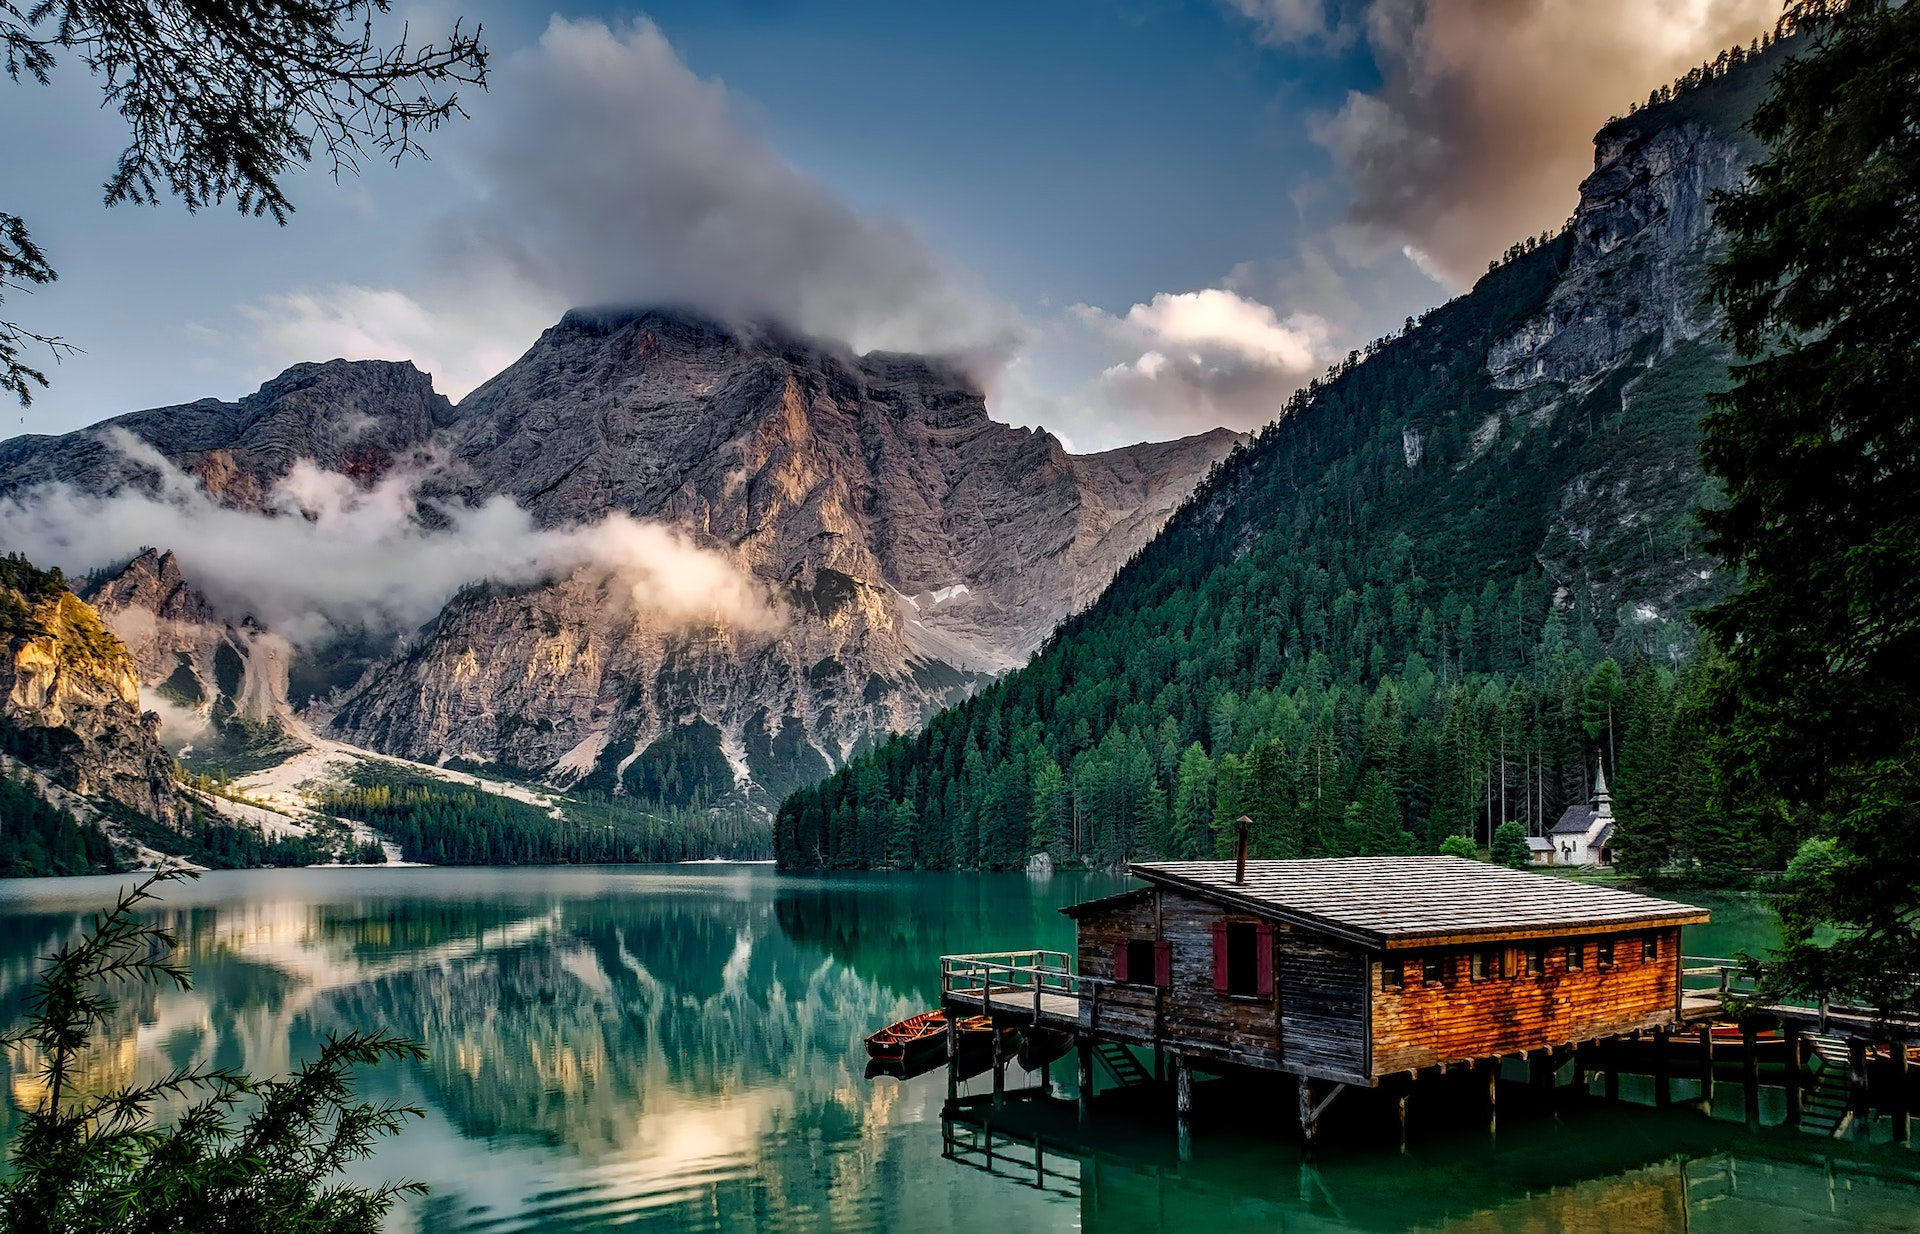
\includegraphics[width=\linewidth]{assets/images/bilder/pexels-pixabay-147411.jpg}
                \subcaption{Holzhütte am Gebirgssee}
            \end{minipage}
            \hfill
            \begin{minipage}[c]{0.49\columnwidth}
                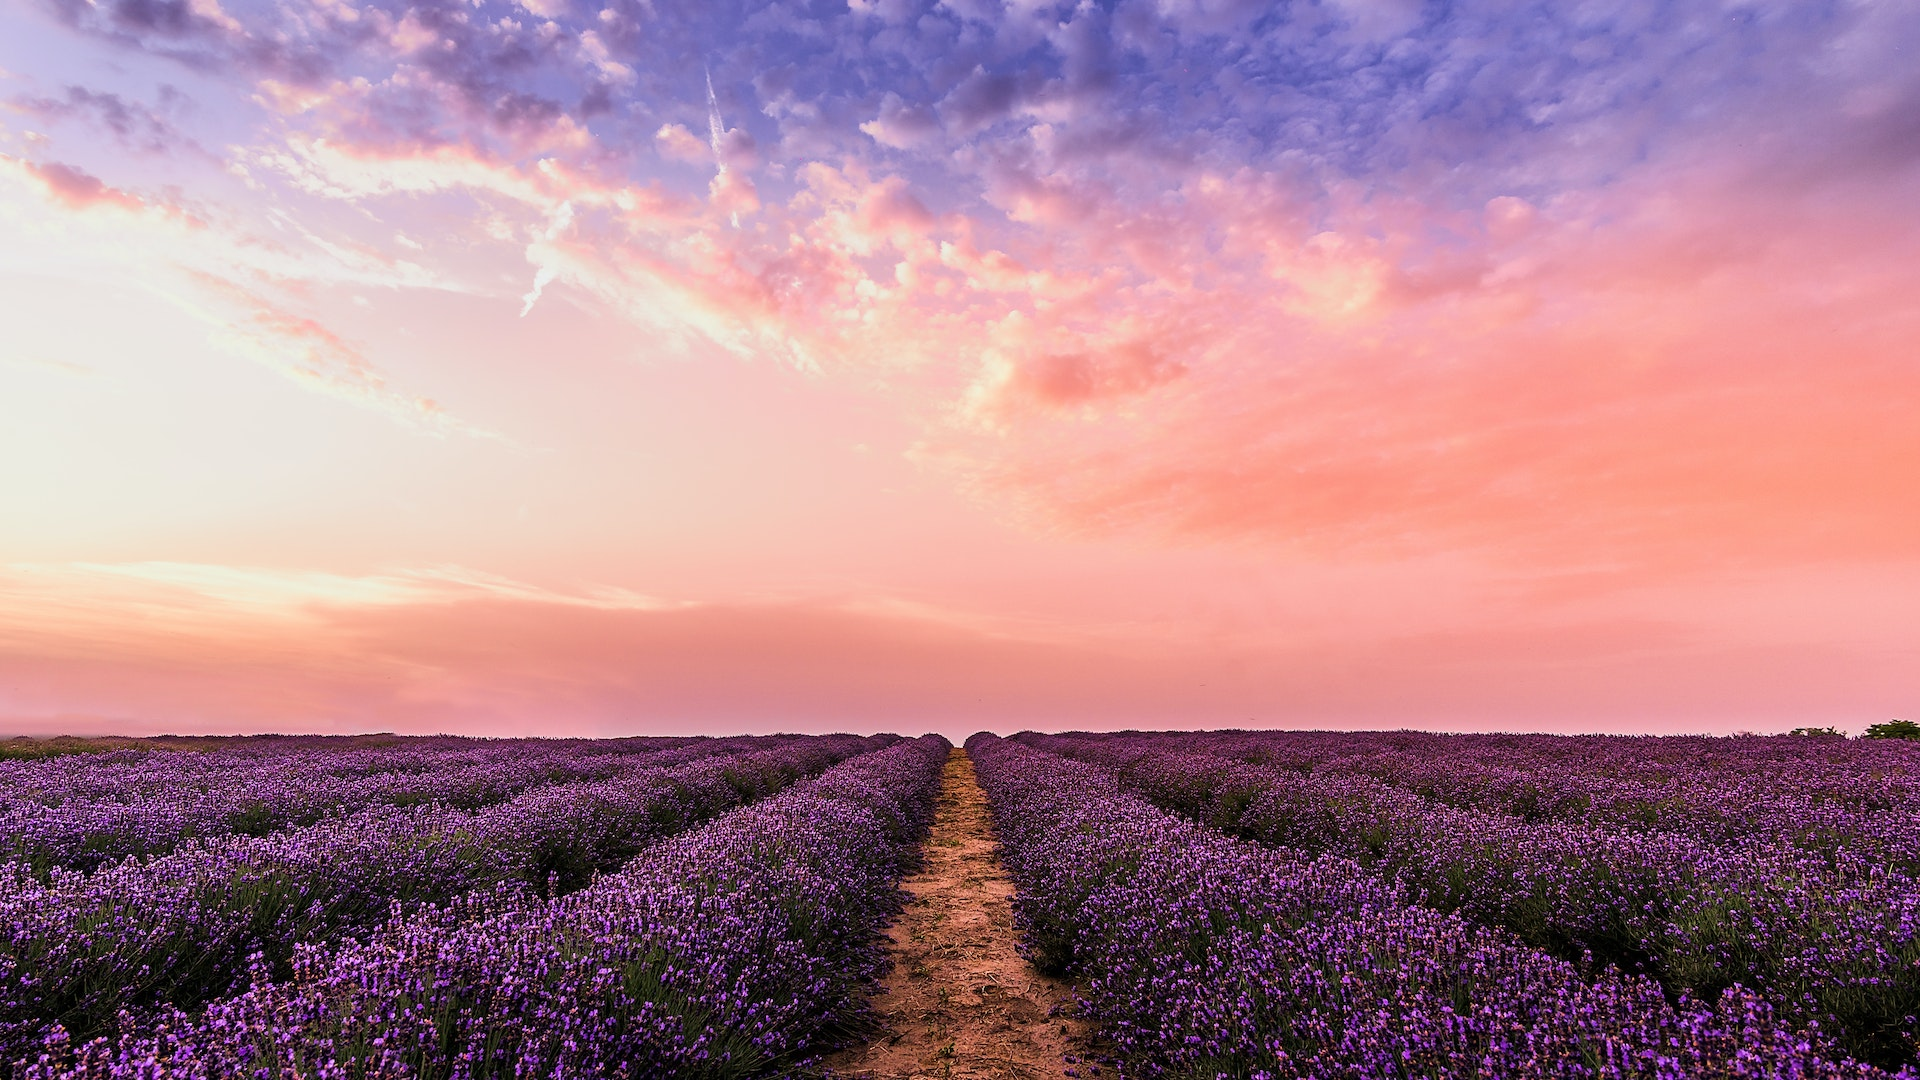
\includegraphics[width=\linewidth]{assets/images/bilder/pexels-david-bartus-1166209.jpg}
                \subcaption{Lavendelfelder im Sonnenuntergang}
            \end{minipage}
            \caption{Zwei farbenprächtige Naturfotografien}
        \end{figure}
    \end{code}
    \tcblower
    \begin{center}
        \captionsetup{type=figure}
        \begin{subfigure}{0.49\columnwidth}
            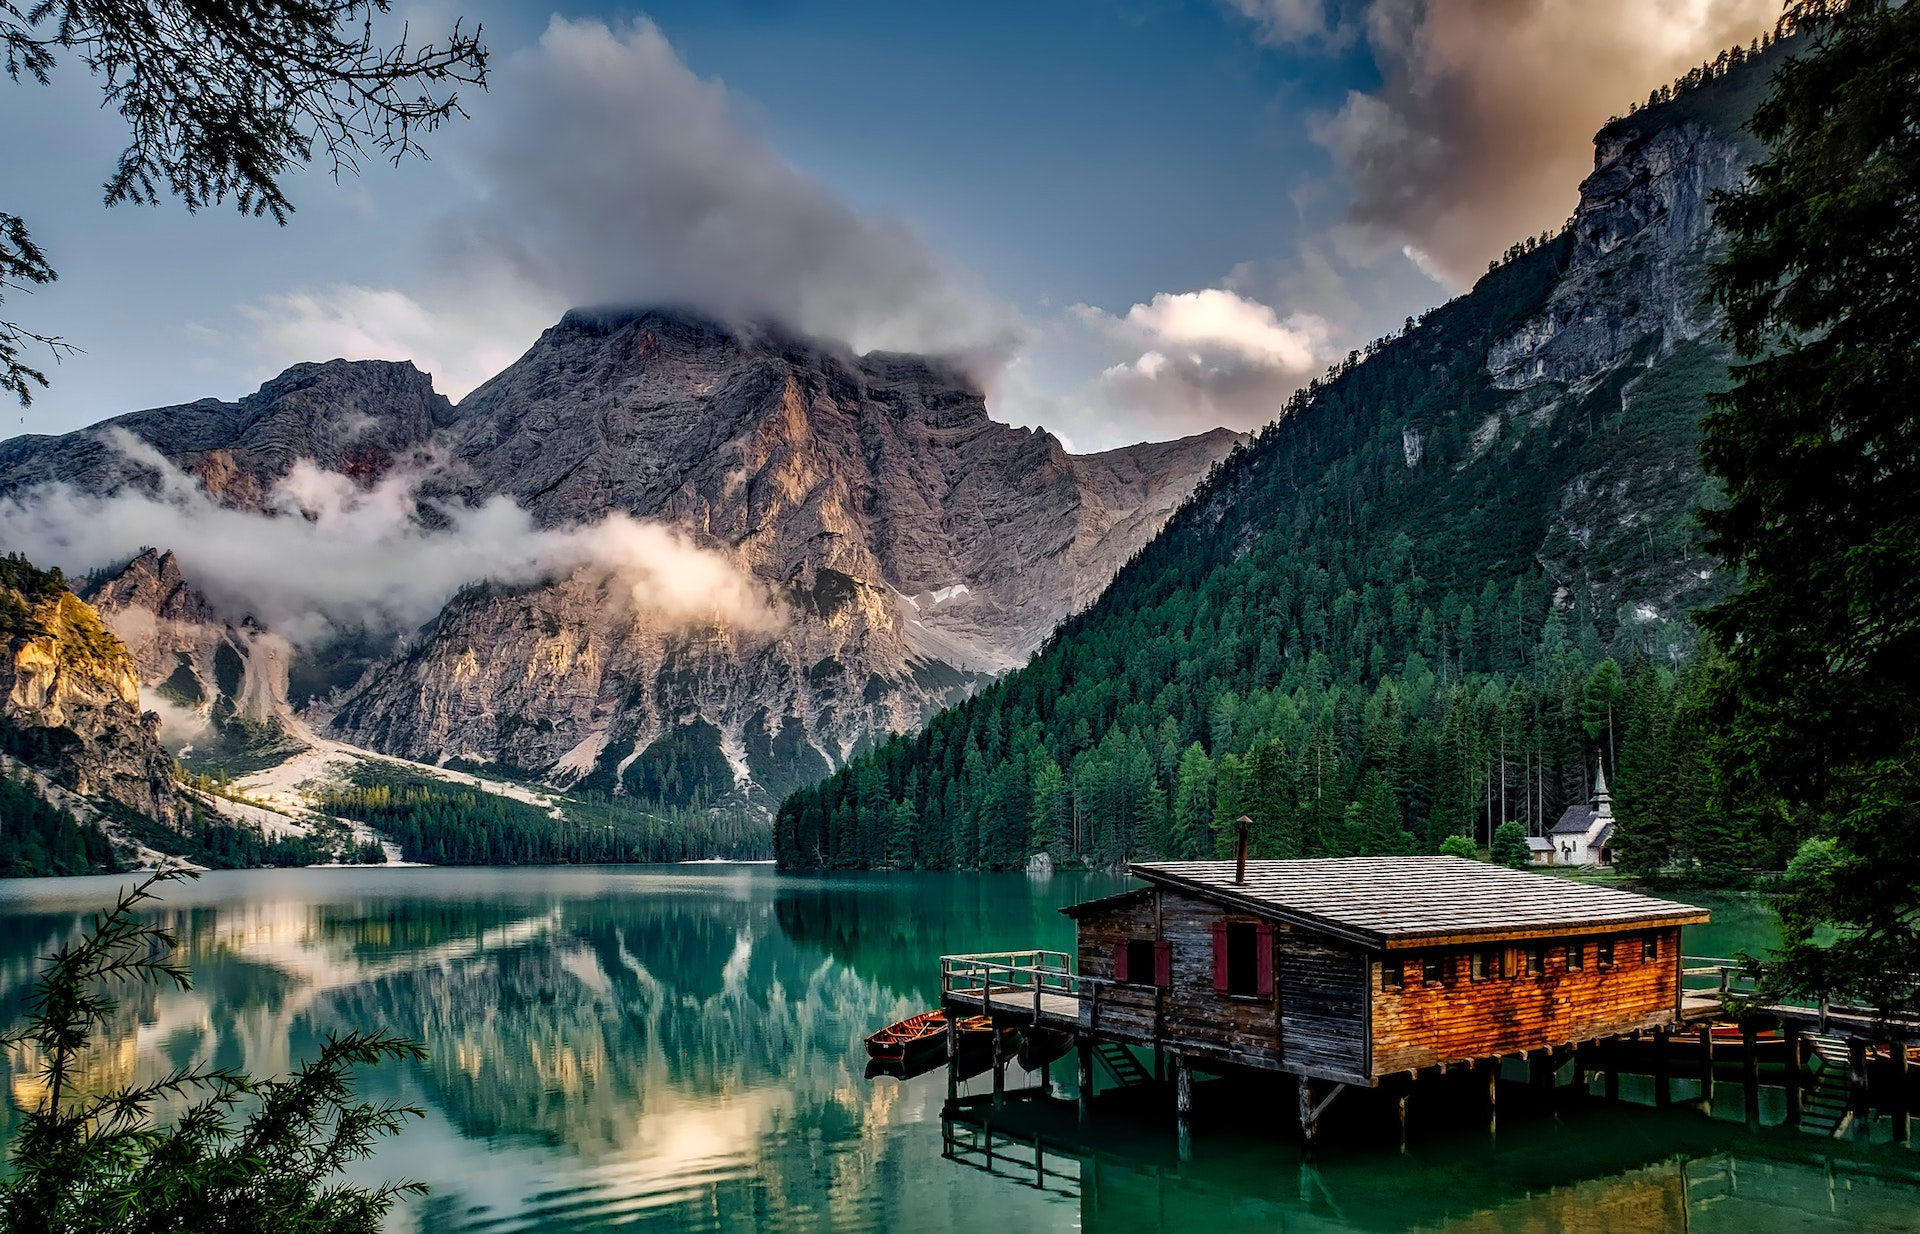
\includegraphics[width=\linewidth]{assets/images/bilder/pexels-pixabay-147411.jpg}
            \caption{Holzhütte am Gebirgssee}
        \end{subfigure}
        \hfill
        \begin{subfigure}{0.49\columnwidth}
            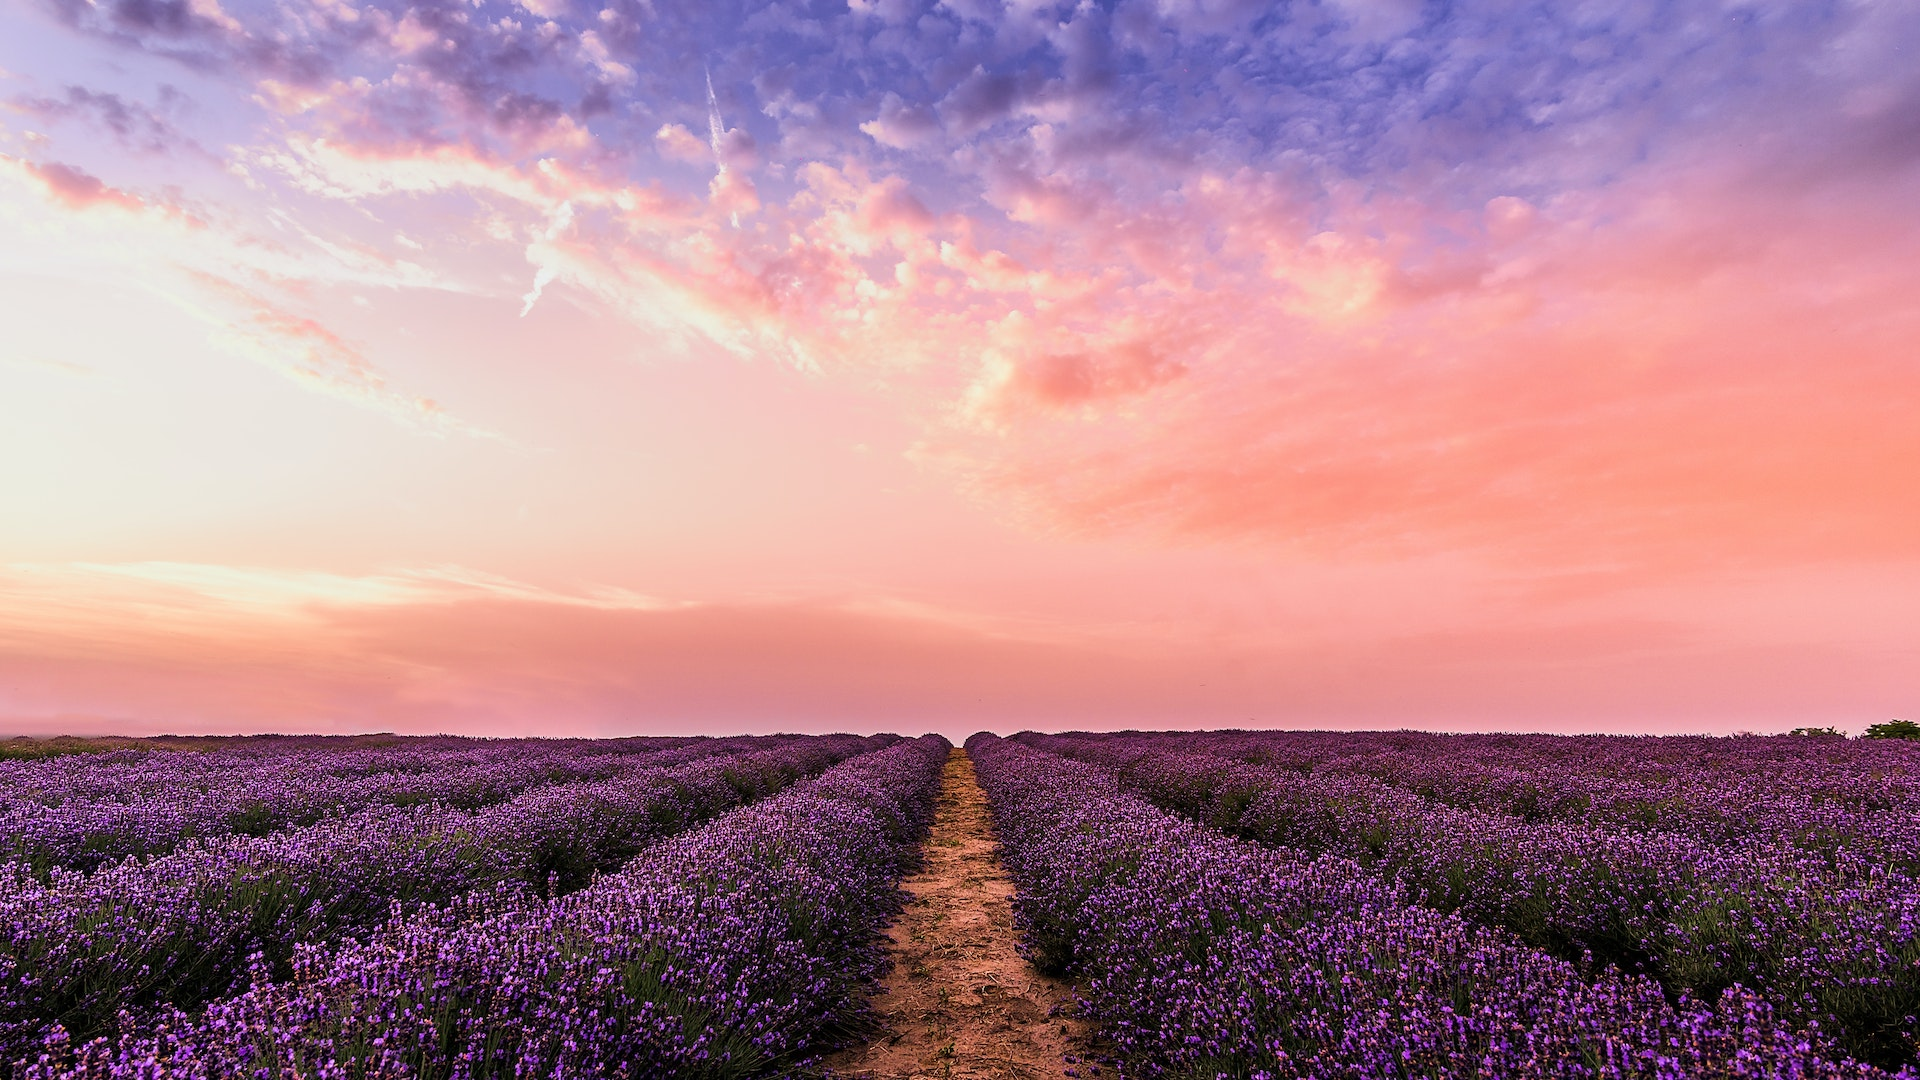
\includegraphics[width=\linewidth]{assets/images/bilder/pexels-david-bartus-1166209.jpg}
            \caption{Lavendelfelder im Sonnenuntergang}
        \end{subfigure}
        \captionof{figure}{Zwei farbenprächtige Landschaftsfotos}
    \end{center}
\end{showcase}

\begin{showcase}
    \begin{code}{latex}
        \begin{figure}[H]
            \begin{minipage}[c]{0.27\columnwidth}
                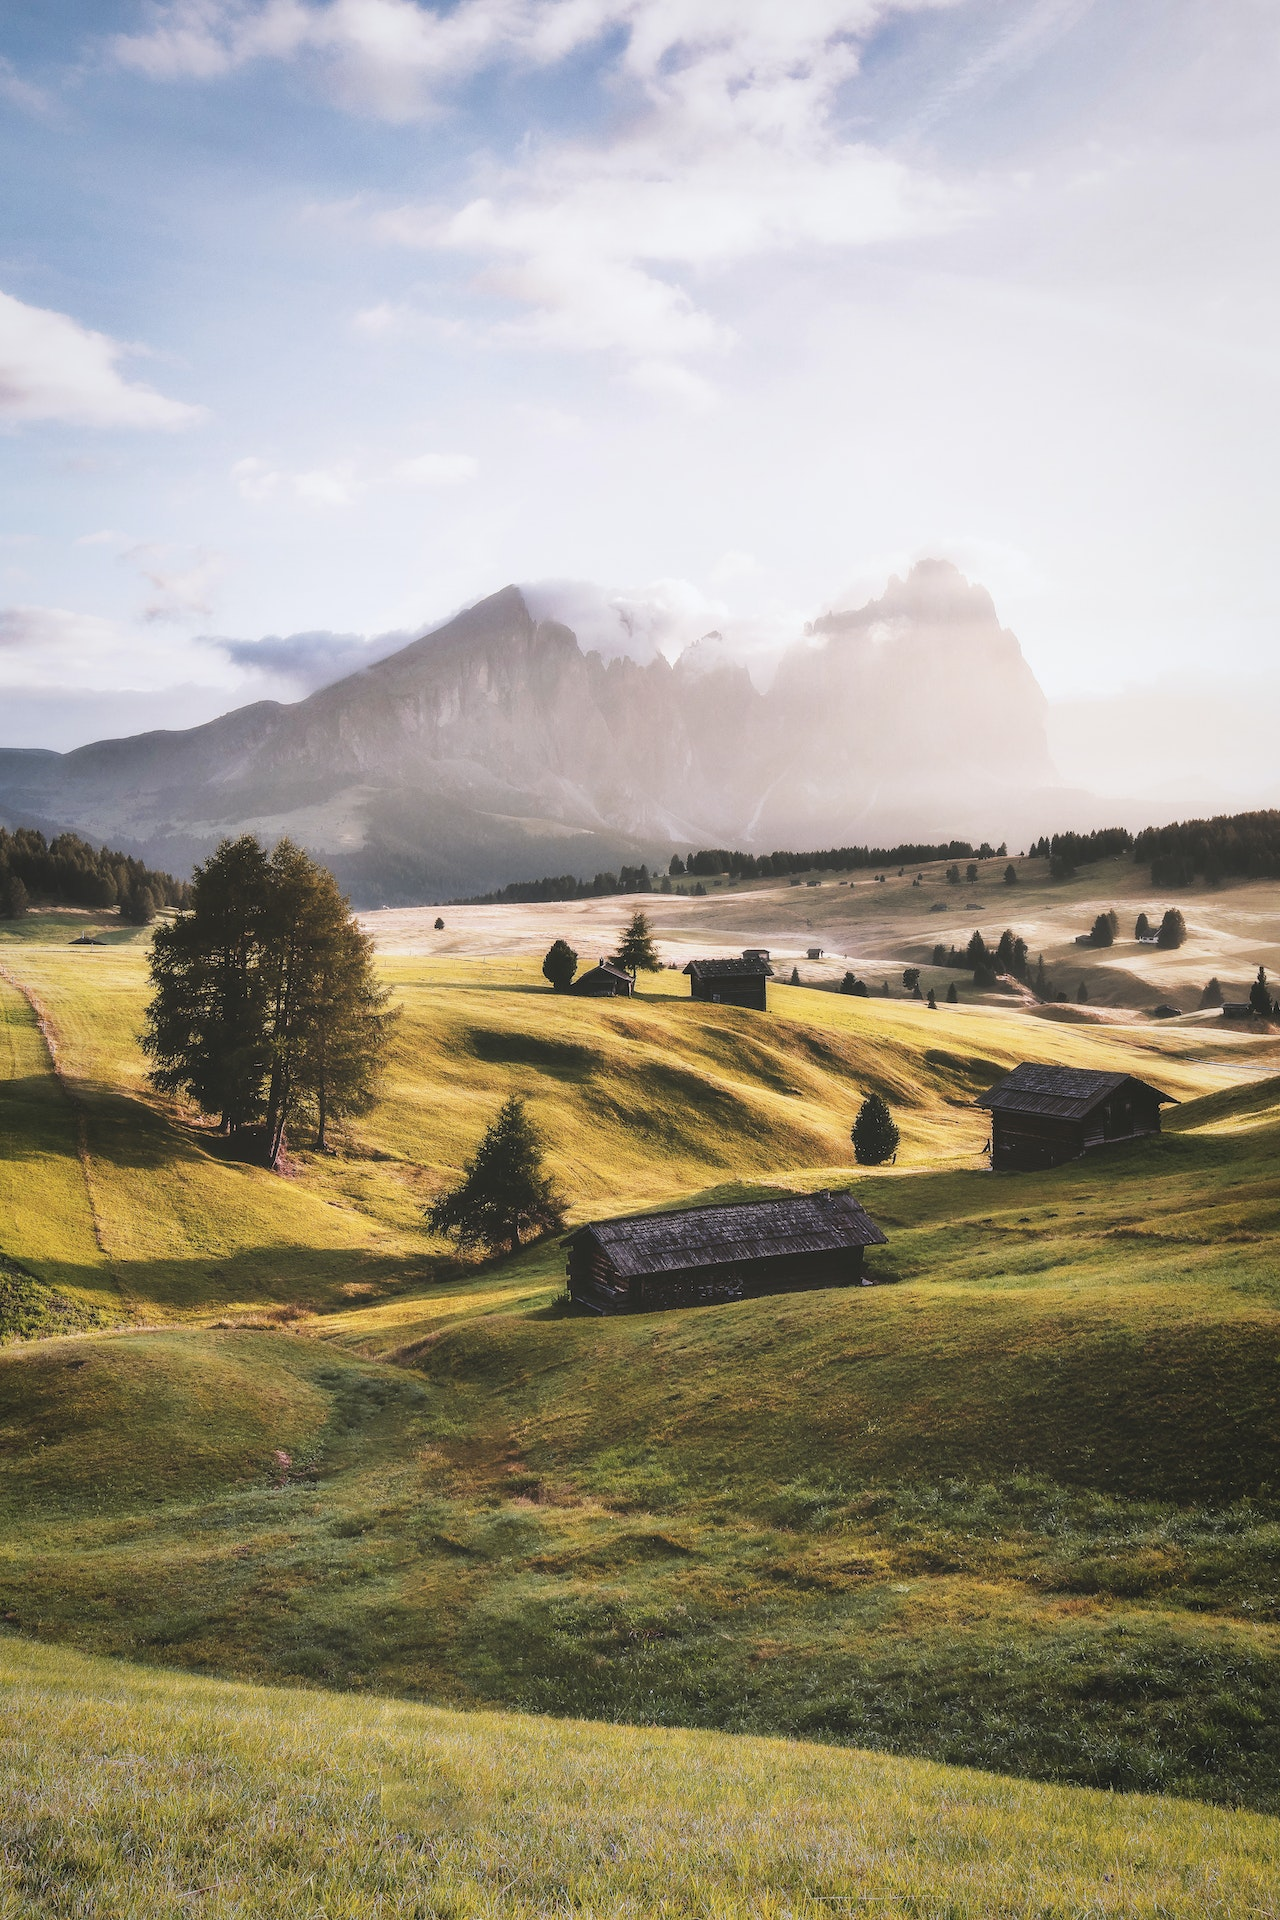
\includegraphics[width=\linewidth,height=6cm,keepaspectratio]{assets/images/bilder/pexels-eberhard-grossgasteiger-2437291.jpg}
                \subcaption{Hügelige Landschaft}
            \end{minipage}
            \hfill
            \begin{minipage}[c]{0.72\columnwidth}
                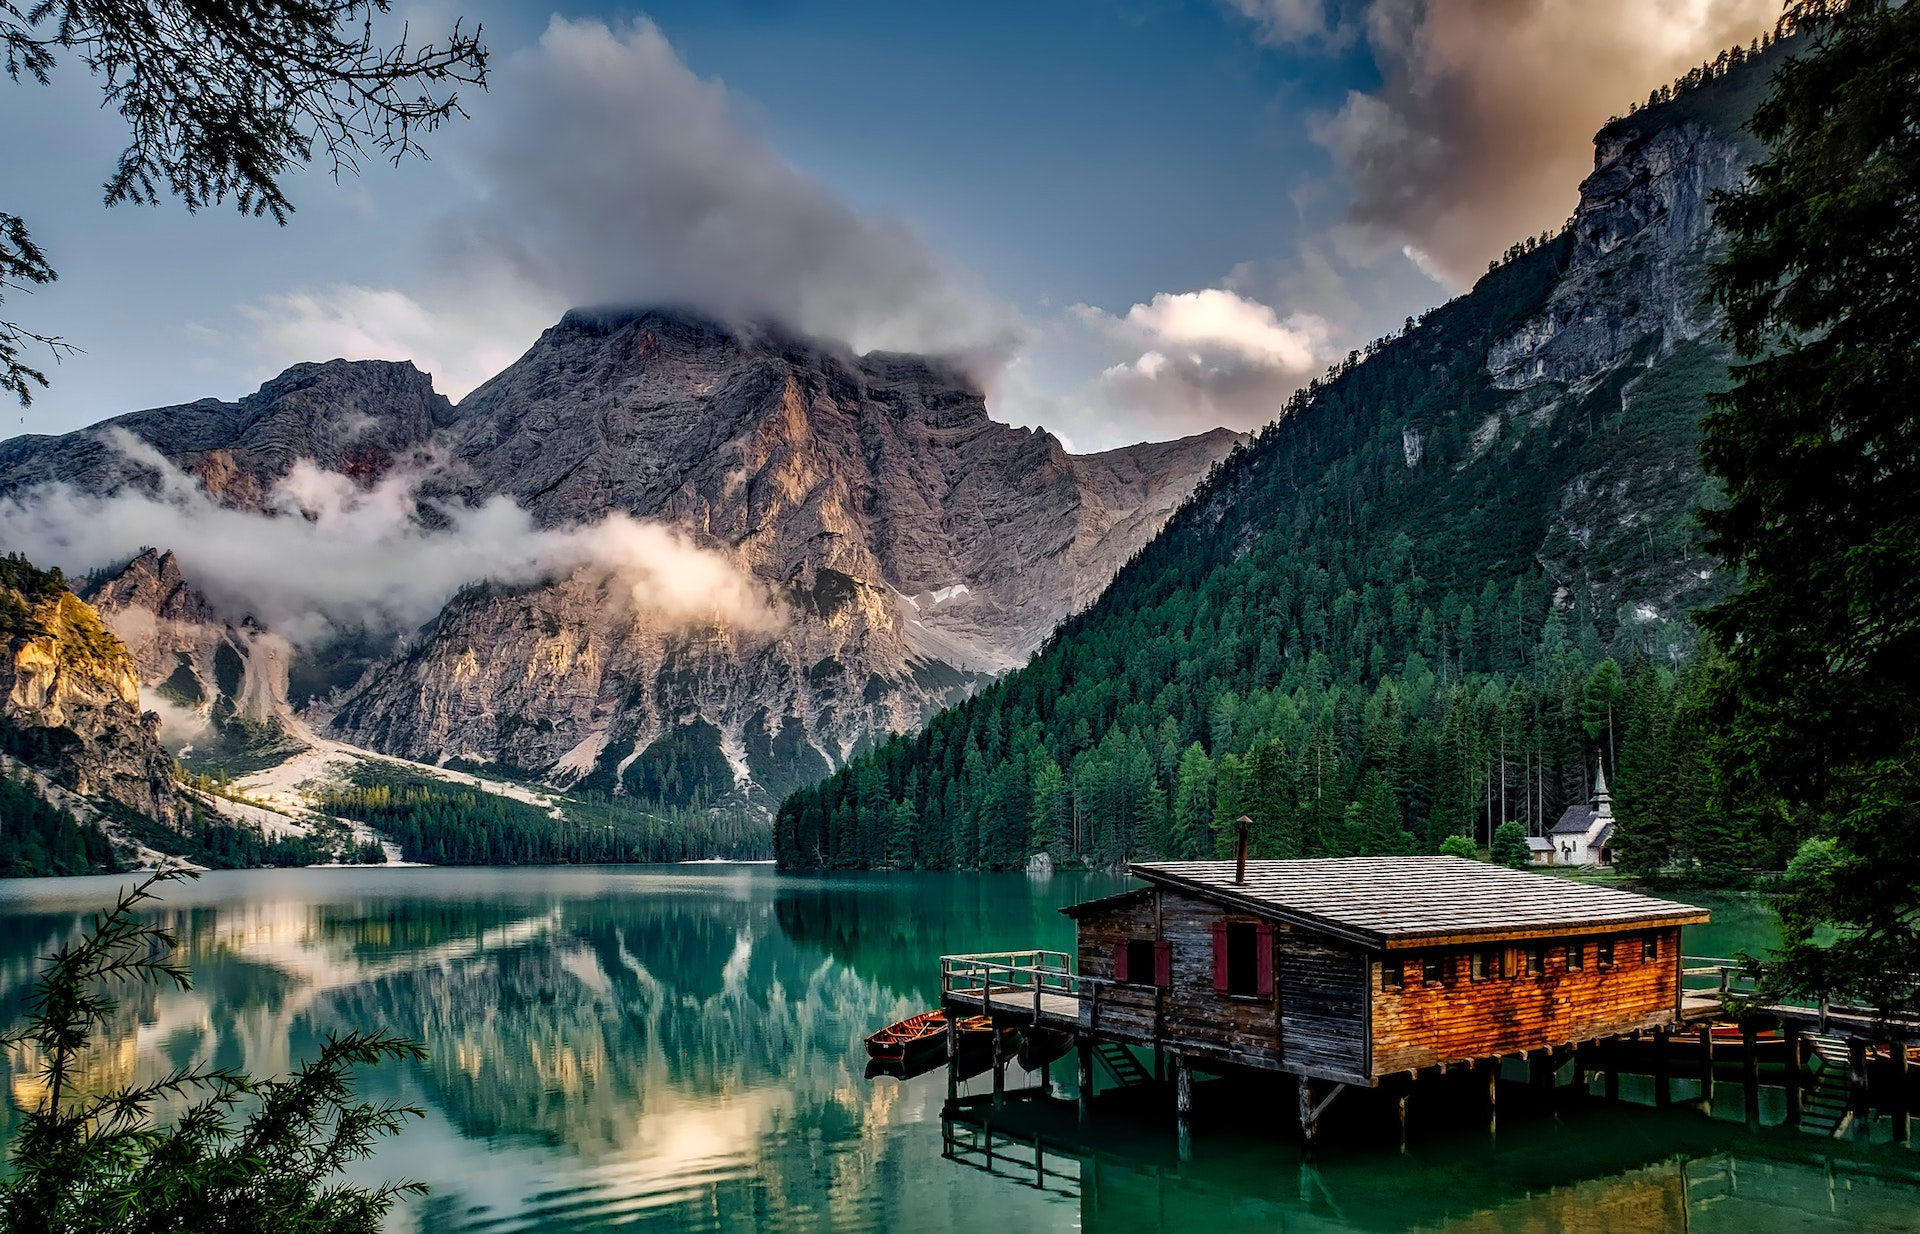
\includegraphics[width=\linewidth,height=6cm,keepaspectratio]{assets/images/bilder/pexels-pixabay-147411.jpg}
                \subcaption{Holzhütte am Gebirgssee}
            \end{minipage}
            \caption{Zwei farbenprächtige Landschaftsfotos}
        \end{figure}
    \end{code}
    \tcblower
    \begin{center}
        \captionsetup{type=figure}
        \begin{subfigure}{0.27\columnwidth}
            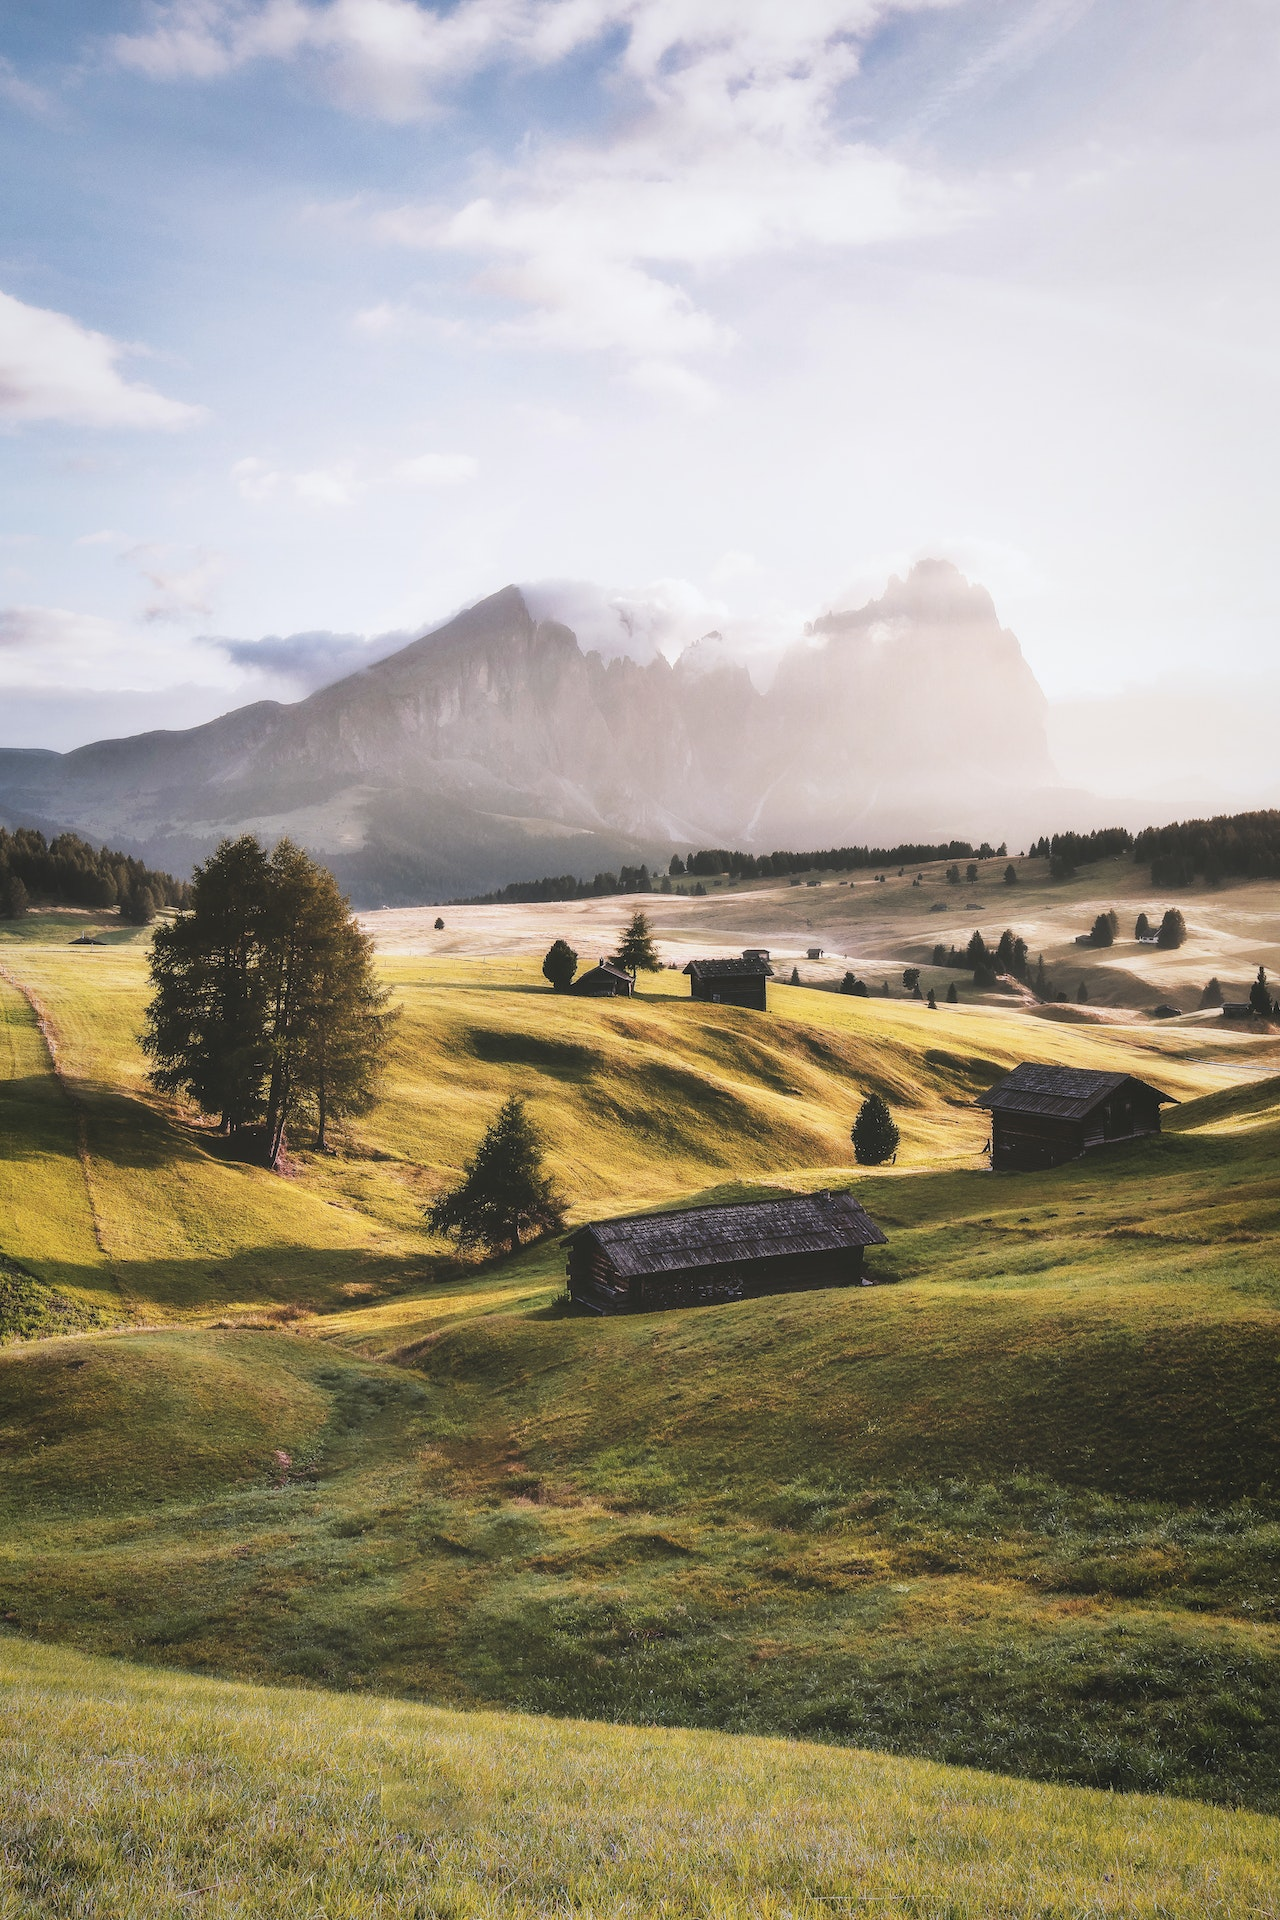
\includegraphics[width=\linewidth,height=6cm,keepaspectratio]{assets/images/bilder/pexels-eberhard-grossgasteiger-2437291.jpg}
            \caption{Hügelige Landschaft}
        \end{subfigure}
        \hfill
        \begin{subfigure}{0.72\columnwidth}
            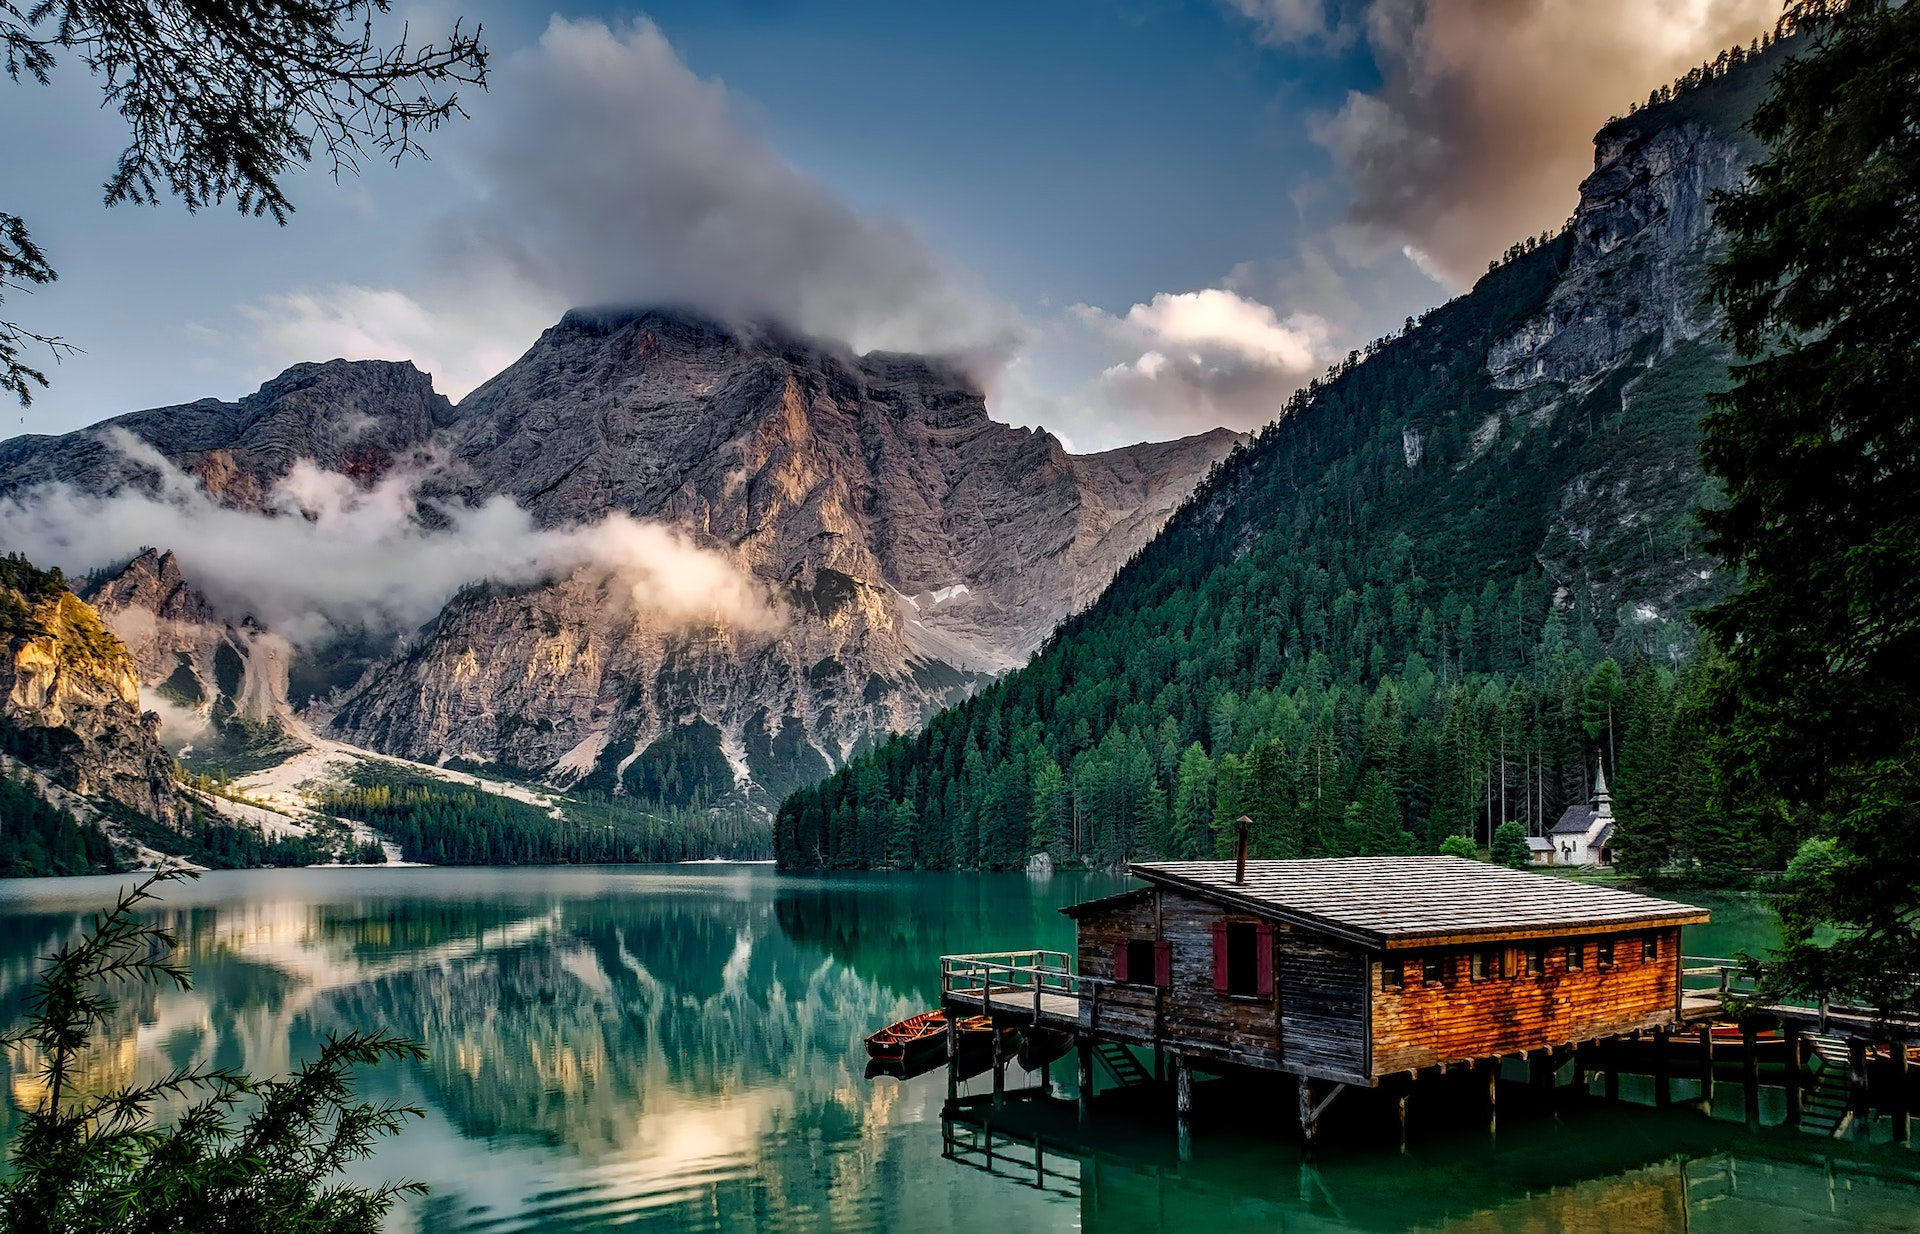
\includegraphics[width=\linewidth,height=6cm,keepaspectratio]{assets/images/bilder/pexels-pixabay-147411.jpg}
            \caption{Holzhütte am Gebirgssee}
        \end{subfigure}
        \captionof{figure}{Zwei farbenprächtige Landschaftsfotos}
    \end{center}
\end{showcase}

\section{Wrapfigure}
Die \texttt{wrapfigure}-Umgebung in \LaTeX ermöglicht es, Bilder in den Textfluss einzufügen und den umgebenden Text harmonisch um die Abbildung zu positionieren. Im Gegensatz zu herkömmlichen Fließumgebungen, die eine separate Zeile für Abbildungen reservieren, kann \texttt{wrapfigure} das Bild links oder rechts vom Text umfließen lassen. Dies ist besonders nützlich, wenn ein Bild eng mit dem umgebenden Text verbunden ist und eine nahtlose Integration gewünscht ist. Wie in einer normalen Fließumgebung können Beschriftungen mit \mintinline{latex}{\caption{}} gesetzt werden. Die Verwendung von \texttt{wrapfigure}-Umgebung erfordert eine sorgfältige Handhabung, da sie den Textfluss beeinflussen kann. Sie sollte mit Bedacht verwendet werden, um sicherzustellen, dass der Lesefluss und das Layout des Dokuments nicht gestört werden. Für weitere Informationen siehe \url{https://ctan.org/pkg/wrapfig2}.

\begin{table}[H]
    \centering
    \captionabove{Optionen für \texttt{wrapfigure} und \texttt{wraptable}}
    \begin{tblr}{lll}
        \toprule
        \SetCell[c=2]{c}\textbf{Option} & & \textbf{Platzierung} \\
        \midrule
        r & R & rechts, fließend rechts \\
        l & L & links, fließend links \\
        i & I & Innenseite, fließend Innenseite  \\
        o & O & Außenseite, fließend Außenseite \\
        \bottomrule
    \end{tblr}
\end{table}

\begin{showcase}
    …
    \begin{code}{latex}
        \begin{wrapfigure}{r}{0.5\columnwidth}
            \centering
            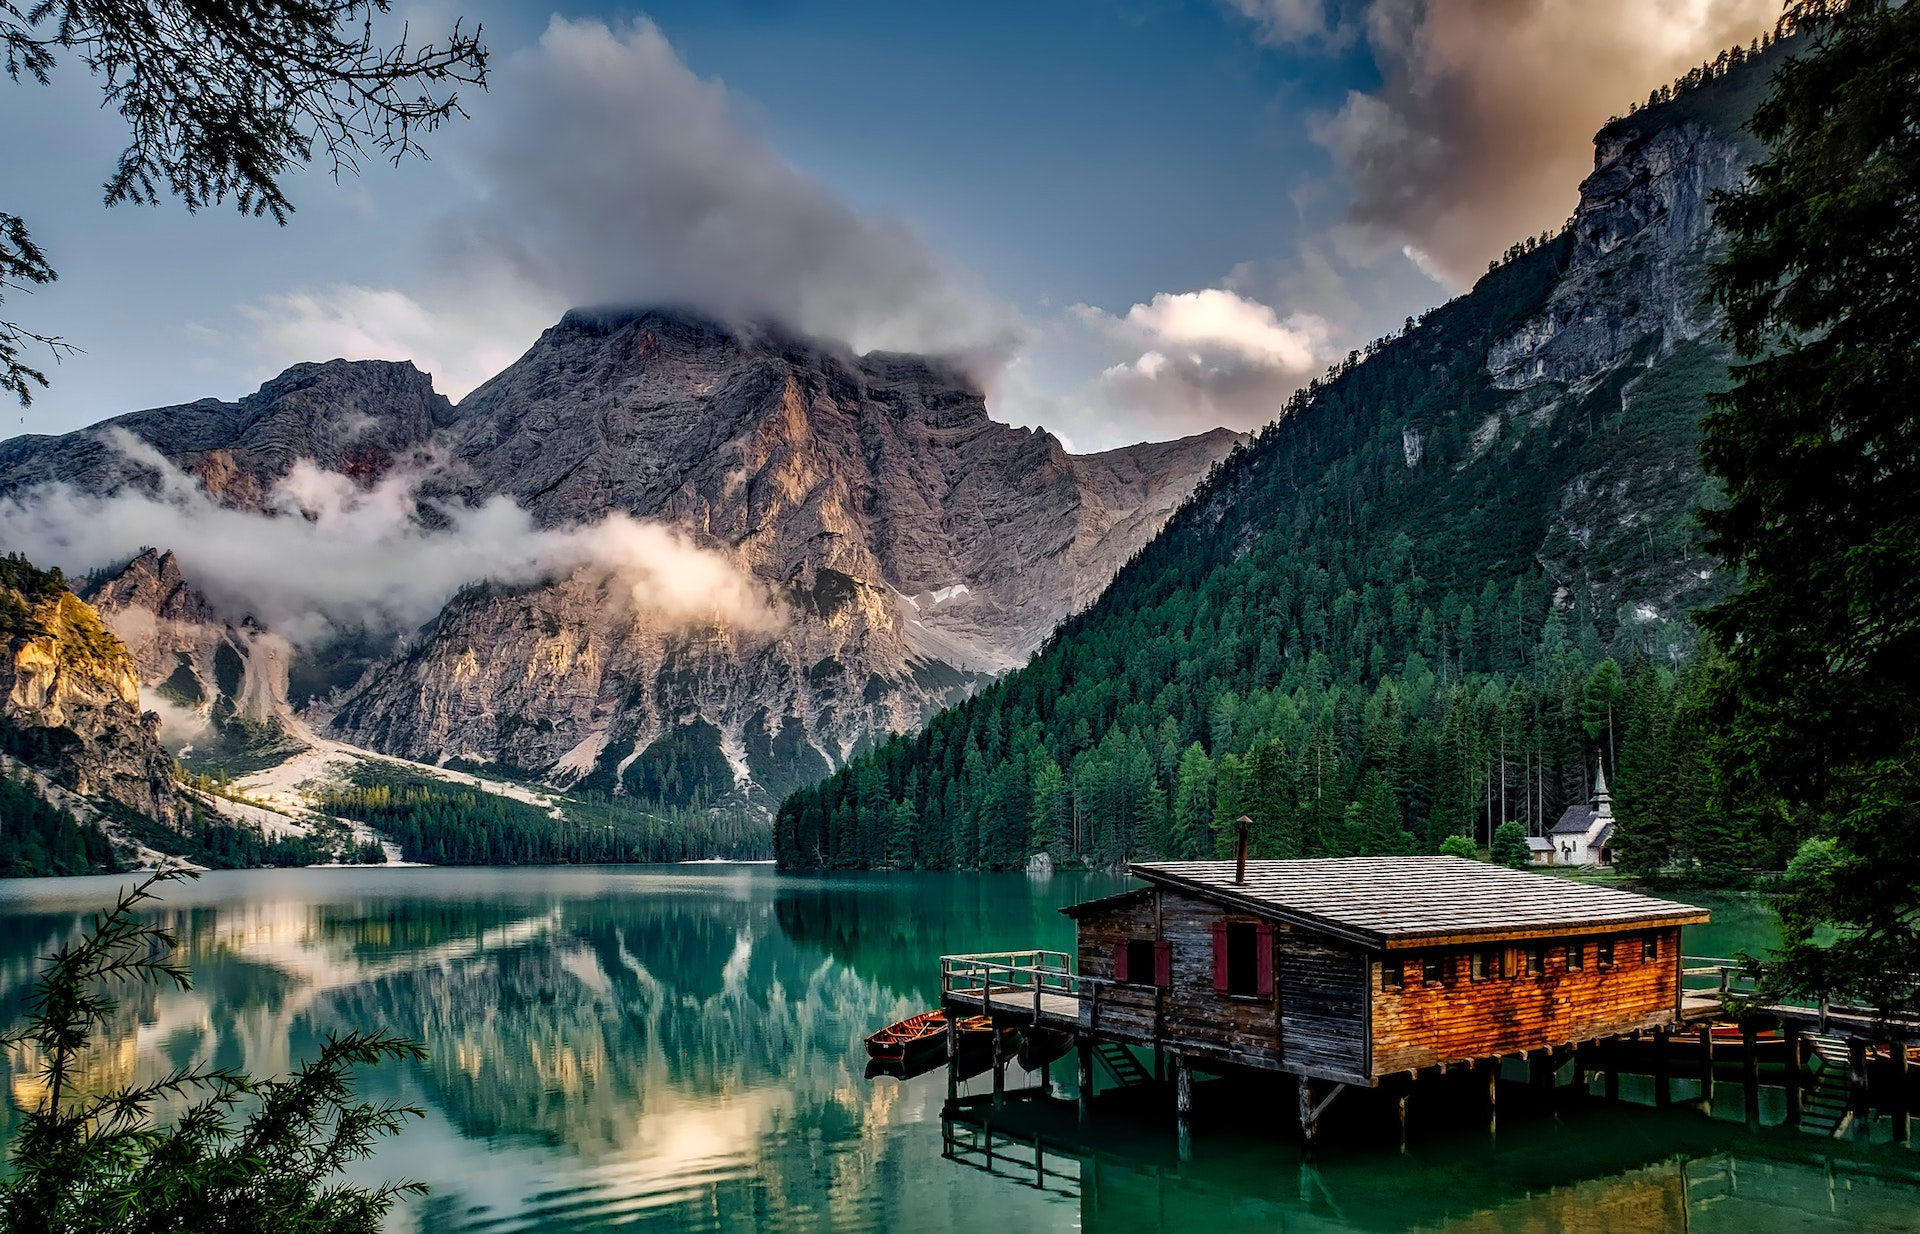
\includegraphics[width=0.5\columnwidth]{assets/images/bilder/pexels-pixabay-147411.jpg}
        \end{wrapfigure}
    \end{code}
    …
    \tcblower
    \begin{wrapfigure}{r}{0.5\columnwidth}
        \centering
        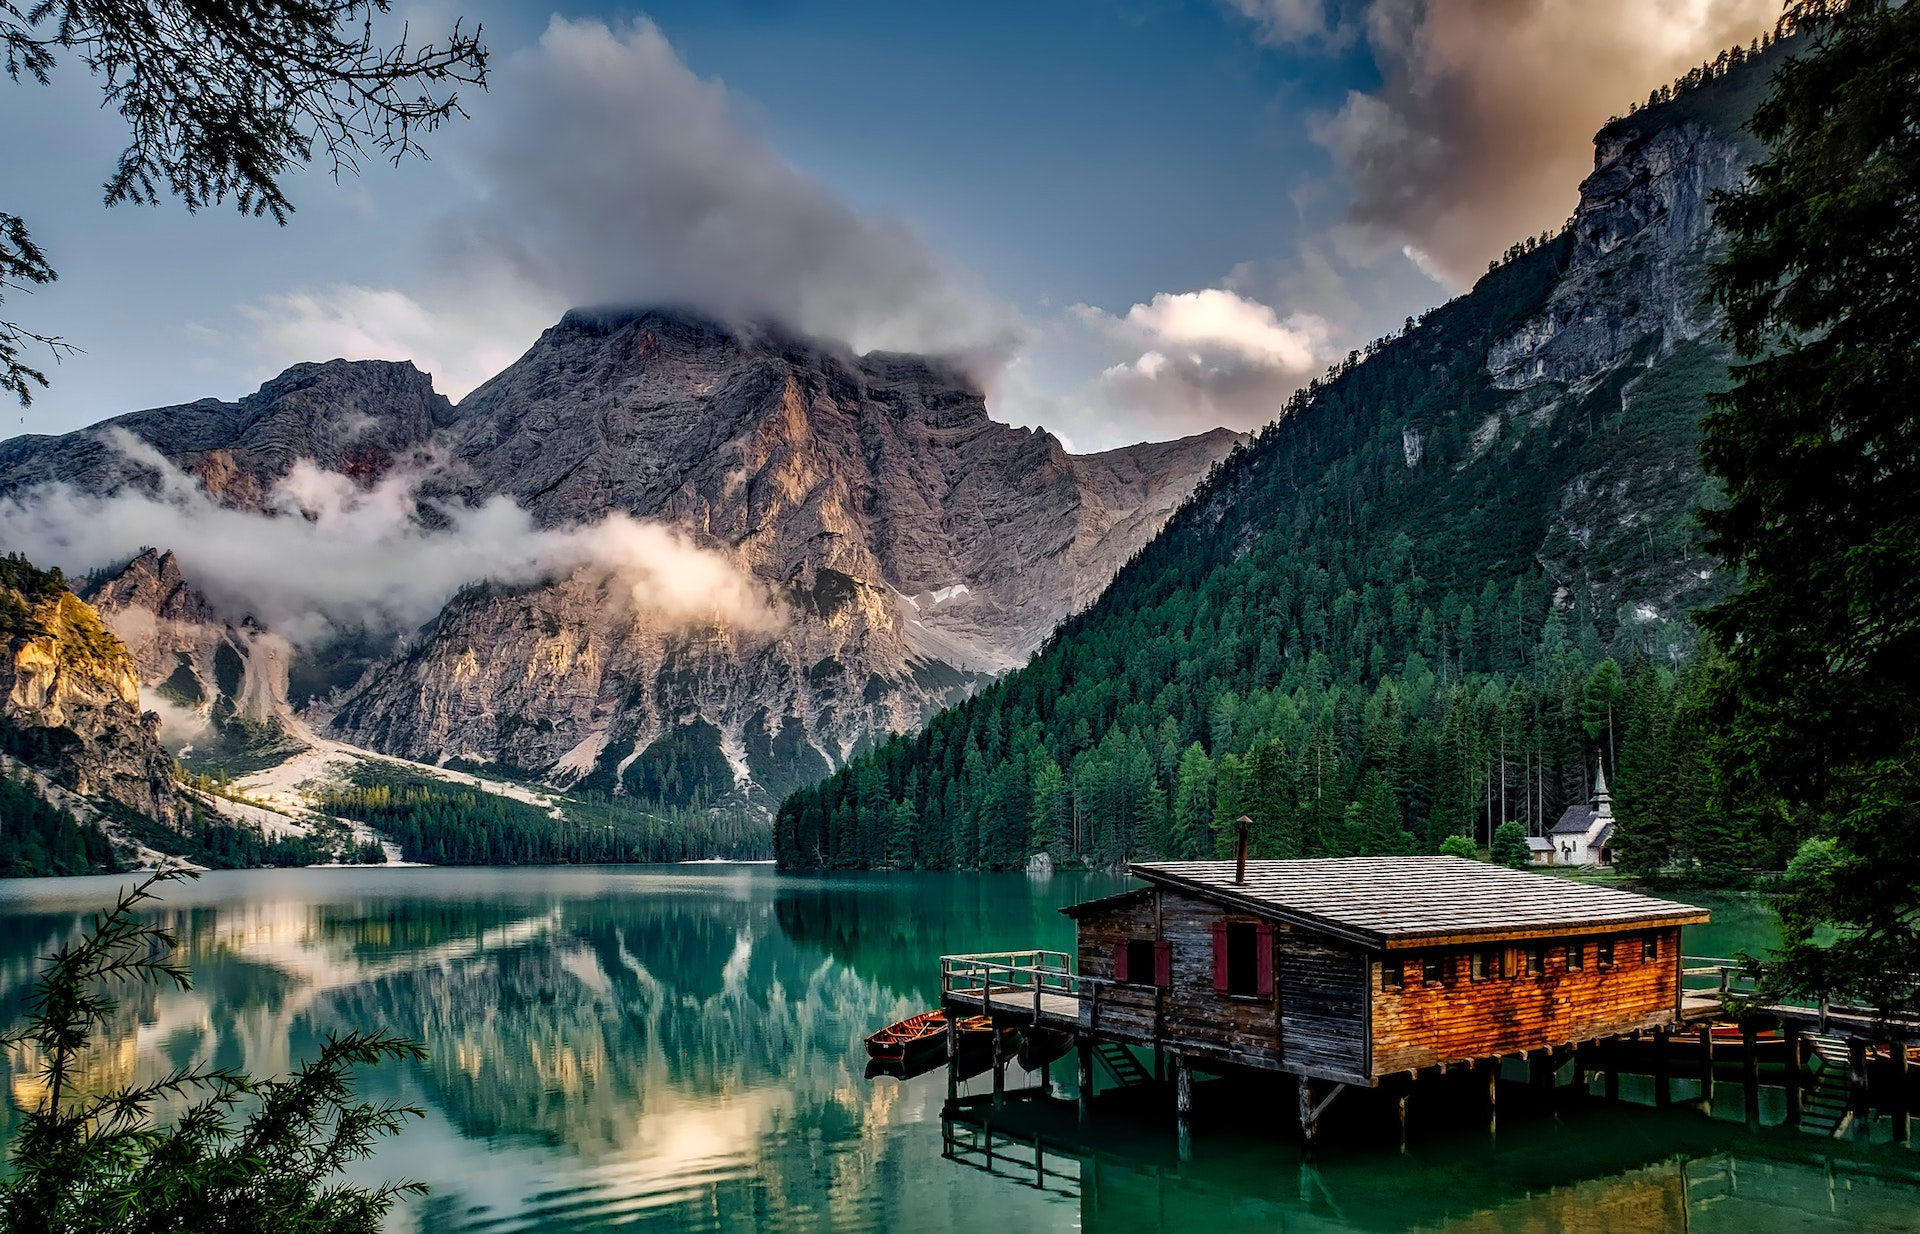
\includegraphics[width=0.5\columnwidth]{assets/images/bilder/pexels-pixabay-147411.jpg}
        \caption{Hütte am See vor dem Kursivgebirge}
    \end{wrapfigure}
    Weit hinten, hinter den Wortbergen, fern der Länder Vokalien und Konsonantien leben die Blindtexte. Abgeschieden wohnen sie in Buchstabhausen an der Küste des Semantik, eines großen Sprachozeans. Nicht einmal von der allmächtigen Interpunktion werden die Blindtexte beherrscht – ein geradezu unorthographisches Leben. Eines Tages aber beschloß eine kleine Zeile Blindtext, ihr Name war Lorem Ipsum, hinaus zu gehen in die weite Grammatik. Der große Oxmox riet ihr davon ab, da es dort wimmele von bösen Kommata, wilden Fragezeichen und hinterhältigen Semikoli, doch das Blindtextchen ließ sich nicht beirren. Es packte seine sieben Versalien, schob sich sein Initial in den Gürtel und machte sich auf den Weg. Als es die ersten Hügel des Kursivgebirges erklommen hatte, warf es einen letzten Blick zurück auf die Skyline seiner Heimatstadt Buchstabhausen, die Headline von Alphabetdorf und die Subline seiner eigenen Straße, der Zeilengasse. Wehmütig lief ihm eine rhetorische Frage über die Wange, dann setzte es seinen Weg fort.
\end{showcase}